% Cover page for Book 2
% Original work by Robert Hildebrand, CC BY-SA 4.0
% Motifs: a branch-and-bound tree (IP algorithms), a nonconvex landscape
% with a descent path (NLP), and a tour with a 2-opt uncrossing (heuristics).
% All elements are drawn in TikZ — no external image dependencies.

\begin{titlepage}
\thispagestyle{empty}
\begingroup
\pagecolor{white}
\centering

\vspace*{0.5in}

{\fontsize{30}{36}\selectfont\bfseries
  Mathematical Programming\\[2pt]
  and Operations Research\par}

\vspace{0.25in}

{\fontsize{14}{18}\selectfont\itshape
  Book 2: Integer and Nonlinear Programming\\
  with Examples in Python and Excel\par}

\vspace{0.5in}

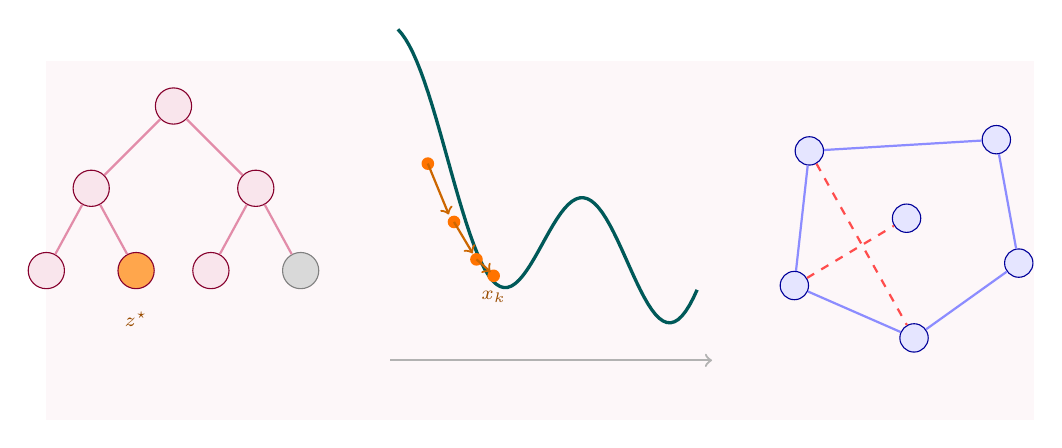
\begin{tikzpicture}[scale=0.95, every node/.style={font=\sffamily\small}]
  \fill[purple!3] (-6.6,-1.2) rectangle (6.6,3.6);

  %% ---------- LEFT: branch-and-bound tree (IP motif) ----------
  \begin{scope}[shift={(-4.9, 3.0)},
      every node/.style={circle, draw=purple!70!black, fill=purple!10,
        minimum size=4.6mm, inner sep=0pt, font=\scriptsize\sffamily}]
    \node (r)  at (0,0)      {};
    \node (a)  at (-1.1,-1.1) {};
    \node (b)  at (1.1,-1.1)  {};
    \node (a1) at (-1.7,-2.2) {};
    \node[fill=orange!70] (a2) at (-0.5,-2.2) {};
    \node (b1) at (0.5,-2.2)  {};
    \node[fill=gray!30, draw=gray] (b2) at (1.7,-2.2) {};
    \begin{scope}[every edge/.style={draw=purple!45, thick}]
      \path (r) edge (a) (r) edge (b)
            (a) edge (a1) (a) edge (a2)
            (b) edge (b1) (b) edge (b2);
    \end{scope}
    \node[draw=none, fill=none, font=\scriptsize\sffamily, orange!60!black]
      at (-0.5,-2.85) {$z^\star$};
  \end{scope}

  %% ---------- CENTER: nonconvex landscape + descent (NLP motif) ----------
  \begin{scope}[shift={(0, -0.4)}]
    \draw[->, gray!60, thick] (-2.0,0) -- (2.3,0);
    \draw[teal!70!black, very thick, domain=-1.9:2.1, samples=80]
      plot (\x, {1.5 + 0.9*sin(150*\x) + 0.28*\x*\x - 0.55*\x});
    % descent path dots toward the global min
    \foreach \p/\s in {-0.25/3.0, 0.05/2.4, 0.28/1.9, 0.52/1.55, 0.72/1.38}{}
    \fill[orange!90!red] (-1.5,2.63) circle (2.4pt);
    \fill[orange!90!red] (-1.15,1.85) circle (2.4pt);
    \fill[orange!90!red] (-0.85,1.35) circle (2.4pt);
    \fill[orange!90!red] (-0.62,1.13) circle (2.4pt);
    \draw[orange!80!black, ->, thick] (-1.5,2.63) -- (-1.22,1.95);
    \draw[orange!80!black, ->, thick] (-1.15,1.85) -- (-0.9,1.43);
    \draw[orange!80!black, ->, thick] (-0.85,1.35) -- (-0.66,1.18);
    \node[font=\scriptsize\sffamily, below, orange!60!black] at (-0.62,1.06) {$x_k$};
  \end{scope}

  %% ---------- RIGHT: tour with 2-opt uncrossing (heuristics motif) ----------
  \begin{scope}[shift={(4.9, 1.2)},
      every node/.style={circle, draw=blue!60!black, fill=blue!10,
        minimum size=3.6mm, inner sep=0pt}]
    \node (t1) at (-1.3, 1.2) {};
    \node (t2) at ( 1.2, 1.35) {};
    \node (t3) at ( 1.5,-0.3) {};
    \node (t4) at ( 0.1,-1.3) {};
    \node (t5) at (-1.5,-0.6) {};
    \node (t6) at ( 0.0, 0.3) {};
    \begin{scope}[every edge/.style={draw=blue!45, thick}]
      \path (t1) edge (t2) (t2) edge (t3) (t3) edge (t4)
            (t4) edge (t5) (t5) edge (t1);
    \end{scope}
    \draw[red!70, dashed, thick] (t1) -- (t4);
    \draw[red!70, dashed, thick] (t5) -- (t6);
  \end{scope}
\end{tikzpicture}

\vspace{0.35in}

{\scriptsize\sffamily\color{gray!70}
  Integer programming \;\textbullet\; complexity \;\textbullet\;
  heuristics \;\textbullet\; nonlinear optimization\par}

\vspace{0.55in}

{\fontsize{20}{24}\selectfont\bfseries Robert Hildebrand\par}
\vspace{4pt}
{\normalsize Virginia Tech\par}

\vspace{0.4in}

{\small
  An open educational resource\\
  Released under the Creative Commons Attribution--ShareAlike\\
  4.0 International License (CC BY-SA 4.0)\par}

\endgroup
\end{titlepage}
